\documentclass[11pt,a4paper]{article}
\usepackage[margin=25mm,headheight=15pt,footskip=13mm]{geometry}
\usepackage[T1]{fontenc}
\usepackage[utf8]{inputenc}
\usepackage{lmodern,microtype,amsmath,amssymb,amsthm,mathtools}
\usepackage{graphicx,booktabs,array,tabularx,xcolor,tikz}
\usetikzlibrary{arrows.meta,positioning,calc,shapes.geometric}
\usepackage[most]{tcolorbox}
\usepackage{hyperref,fancyhdr,enumitem,caption,needspace}
\definecolor{ink}{HTML}{162C42}
\definecolor{teal}{HTML}{007F80}
\definecolor{soft}{HTML}{E9F5F3}
\definecolor{gold}{HTML}{D79C3A}
\definecolor{mist}{HTML}{F3F6F8}
\definecolor{muted}{HTML}{536879}
\hypersetup{colorlinks=true,linkcolor=teal,citecolor=teal,urlcolor=teal,pdftitle={Goldbach as Geometry, Parity and Correlation},pdfauthor={Christopher Yamba}}
\setlength{\parindent}{0pt}
\setlength{\parskip}{5pt}
\setlength{\emergencystretch}{2em}
\captionsetup{font=small,labelfont={bf,color=ink},textfont=small,skip=6pt}
\pagestyle{fancy}\fancyhf{}\fancyhead[L]{\footnotesize\color{muted}\textsf{THE GOLDBACH RESEARCH PROGRAMME}}\fancyhead[R]{\footnotesize\color{muted}\textsf{RESEARCH EDITION}}\fancyfoot[R]{\footnotesize\color{muted}\thepage}\renewcommand{\headrulewidth}{0pt}
\newtheorem{prop}{Proposition}[section]
\newtheorem{theorem}[prop]{Theorem}
\newtheorem{target}[prop]{Research target}
\newcommand{\PP}{\mathbb P}
\newcommand{\one}{\mathbf 1}
\newcommand{\Om}{\Omega}
\newcommand{\rough}{P^{-}}
\newcommand{\e}{\mathrm e}
\newcommand{\liou}{\lambda}
\newcommand{\R}{\mathcal R}
\newtcolorbox{insight}[1]{enhanced,colback=soft,colframe=teal,boxrule=0pt,leftrule=2pt,arc=0pt,left=10pt,right=10pt,top=7pt,bottom=7pt,title={\textsf{\bfseries #1}},coltitle=ink,colbacktitle=soft,fonttitle=\small}
\newtcolorbox{caution}[1]{enhanced,colback=mist,colframe=ink!28,boxrule=0pt,leftrule=2pt,arc=0pt,left=10pt,right=10pt,top=7pt,bottom=7pt,title={\textsf{\bfseries #1}},coltitle=ink,colbacktitle=mist,fonttitle=\small}
\title{\vspace{-1.5em}\textcolor{teal}{\large\sffamily RESEARCH PROGRAMME}\vspace{.6em}\\\textcolor{ink}{\Huge\bfseries Goldbach as Geometry,\\[.15em]Parity and Correlation}\\[.65em]\large Visual structures and proof targets for the binary problem}
\author{\textbf{Christopher Yamba}\\[-.1em]\small Research programme developed with computational and AI-assisted investigation}
\date{28 October 2026}
\begin{document}
\maketitle
\begin{abstract}
Every even integer greater than two is conjectured to be a sum of two primes. This article develops a visual and analytic research programme around that open question. Prime-pair sums form layers of a Ferrers diagram, reflection matrices encode representations as elementary blocks, and modular sieving becomes a covering problem. A prime-versus-semiprime parity statistic exposes a precise pointwise hurdle; an averaged calculation reveals a cutoff at which the leading balance reverses. The article also describes a classical Buchstab integral, a conditional M\"obius-twisted distribution route, and adversarial examples that test what any proof must use. The mathematical deductions here are working results derived from established inputs and checked computationally or by independent research agents; they have not received external peer review. No proof of Goldbach or claim of priority is made.
\end{abstract}
\begin{caution}{Status and scope}
Goldbach's binary conjecture remains open. All finite checks in this article are evidence about their stated ranges, not proofs at arbitrary size. Terms such as \emph{research target} identify unproved statements. The averages in this article concern ordered pairs; in particular, $p+q$ and $q+p$ count separately when $p\ne q$.
\end{caution}
\vspace{1em}
\begin{center}
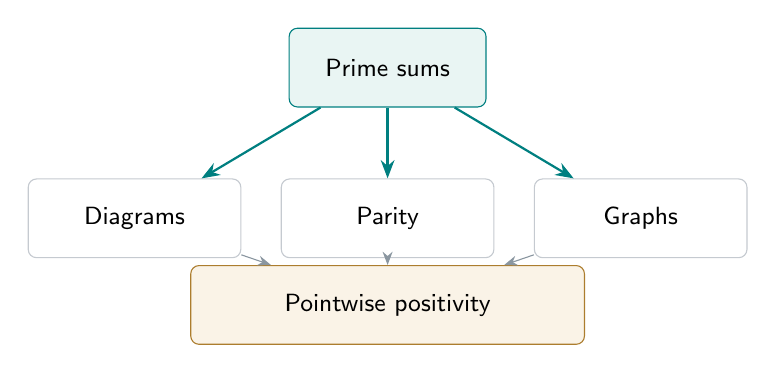
\begin{tikzpicture}[node distance=9mm and 6mm,every node/.style={font=\small\sffamily}]
\node[draw=teal,fill=soft,rounded corners=3pt,minimum width=25mm,minimum height=10mm] (s) {Prime sums};
\node[draw=ink!25,fill=white,rounded corners=3pt,minimum width=27mm,minimum height=10mm,below left=of s] (d) {Diagrams};
\node[draw=ink!25,fill=white,rounded corners=3pt,minimum width=27mm,minimum height=10mm,below=of s] (p) {Parity};
\node[draw=ink!25,fill=white,rounded corners=3pt,minimum width=27mm,minimum height=10mm,below right=of s] (g) {Graphs};
\node[draw=gold!80!black,fill=gold!12,rounded corners=3pt,minimum width=50mm,minimum height=10mm,below=20mm of s] (t) {Pointwise positivity};
\draw[-{Stealth},teal,thick] (s)--(d);\draw[-{Stealth},teal,thick] (s)--(p);\draw[-{Stealth},teal,thick] (s)--(g);
\draw[-{Stealth},ink!50] (d)--(t);\draw[-{Stealth},ink!50] (p)--(t);\draw[-{Stealth},ink!50] (g)--(t);
\end{tikzpicture}
\captionof{figure}{Different languages meet at the same difficult question: can a positive pair count be proved for \emph{each} even target?}
\end{center}
\newpage
\section{A small equation, an exacting demand}
Write
\begin{equation}\label{eq:R}
 R(N)=\#\{p\in\PP: N-p\in\PP\}.
\end{equation}
For even $N\ge4$, the strong Goldbach conjecture asks for $R(N)>0$. For example, $30$ has six ordered representations, coming from $7+23$, $11+19$ and $13+17$ and their reversals. There are no known counterexamples; the published verification by Oliveira e Silva, Herzog and Pardi reaches $4\cdot 10^{18}$ \cite{verification}. Computation does not settle infinitely many cases.

The surrounding landscape is rich. Helfgott proved the ternary conjecture: every odd integer greater than five is a sum of three primes \cite{helfgott}. Chen proved that every sufficiently large even integer is a prime plus a number with at most two prime factors. Both achievements illuminate the binary problem, but neither automatically fixes an arbitrary two-prime slice. The difficulty is especially clear in the difference between a statement about \emph{almost every} even integer and a pointwise statement about \emph{every} one.

\begin{insight}{The central question}
How can we turn abundant average structure into a positive lower bound at one fixed target $N$? Each representation below sharpens this question. None removes it by relabelling alone.
\end{insight}

\section{The geometry of prime sums}
List the odd primes $p_1<p_2<\cdots$ and form the set
\begin{equation}\label{eq:ferrers}
 \mathcal F_2(N)=\{(i,j):p_i+p_j\le N\}.
\end{equation}
It is a Ferrers diagram: if a box appears, every box weakly above and to its left appears too. The difference $\mathcal F_2(N)\setminus\mathcal F_2(N-2)$ consists exactly of the ordered representations of $N$ by odd primes. For even $N\ge6$ this is all of $R(N)$; the exceptional case $4=2+2$ is handled separately.

\begin{figure}[htbp]
\centering
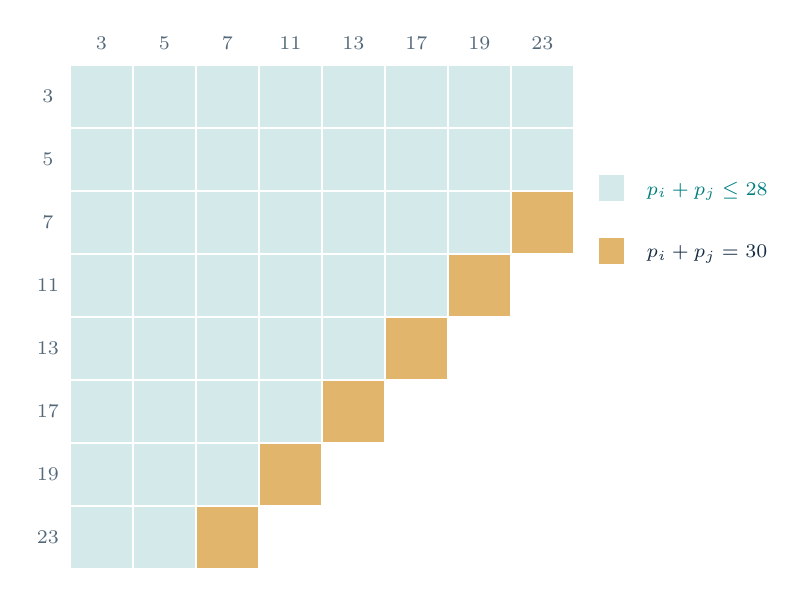
\begin{tikzpicture}[x=8mm,y=8mm]
\def\primes{{3,5,7,11,13,17,19,23}}
\foreach \i in {0,...,7}{\foreach \j in {0,...,7}{
\pgfmathtruncatemacro{\a}{\primes[\i]}\pgfmathtruncatemacro{\b}{\primes[\j]}
\pgfmathtruncatemacro{\v}{\a+\b}
\ifnum\v<30 \fill[teal!17] (\j,-\i) rectangle +(1,-1);\else\ifnum\v=30 \fill[gold!75] (\j,-\i) rectangle +(1,-1);\fi\fi
\draw[white,line width=.7pt] (\j,-\i) rectangle +(1,-1);
}}
\foreach \i/\p in {0/3,1/5,2/7,3/11,4/13,5/17,6/19,7/23}{\node[font=\scriptsize,color=muted] at (\i+.5,.35) {\p};\node[font=\scriptsize,color=muted] at (-.35,-\i-.5) {\p};}
\node[font=\scriptsize,color=teal,anchor=west] at (9,-2) {$p_i+p_j\le28$};
\fill[teal!17] (8.4,-2.15) rectangle +(0.4,0.4);
\node[font=\scriptsize,color=ink,anchor=west] at (9,-3) {$p_i+p_j=30$};
\fill[gold!75] (8.4,-3.15) rectangle +(0.4,0.4);
\end{tikzpicture}
\caption{Prime-index Ferrers diagram at $30$. Gold squares are the new layer. Row and column labels are prime values, not consecutive integers.}
\label{fig:ferrers}
\end{figure}

Every row and every column contains at most one new box. Thus the layer is a symmetric placement of nonattacking rooks. A diagonal box is the special case $N=2p$, where $p$ is prime. For arbitrary Ferrers diagrams a layer may be empty; the unanswered question is what additional property of the \emph{prime-index} family forbids an empty even layer.

The construction extends naturally to
\[
 \mathcal F_k(T)=\{(i_1,\ldots,i_k):p_{i_1}+\cdots+p_{i_k}\le T\}.
\]
Each new shell is a partial Latin-hypercube pattern: an axis-parallel line contains at most one new box. The two-prime problem for $N$ can be viewed as the slice of the three-prime shell at $N+3$ whose third coordinate is $3$. A nonempty three-dimensional shell need not intersect that specific slice. This is a geometric picture of why a ternary theorem does not immediately establish the binary one.

\section{Reflection, permutations and graphs}
Let $D$ be diagonal on the integers $2,\ldots,N-2$, with $D_{aa}=1$ for primes and zero otherwise. Let $J_N$ be the permutation that reflects $a$ to $N-a$. The symmetric matrix
\[
 B_N=D J_N D
\]
retains exactly those reflection edges whose endpoints are both prime. Every unequal Goldbach pair contributes a block $\bigl(\begin{smallmatrix}0&1\\1&0\end{smallmatrix}\bigr)$; a pair $p+p=N$ contributes the block $(1)$. Therefore
\begin{equation}\label{eq:trace}
 R(N)=\operatorname{tr}(B_N^2)=2k+f,
\end{equation}
where $k$ is the number of unequal unordered pairs and $f=1$ if $N/2$ is prime, otherwise $0$.

\begin{figure}[htbp]
\centering
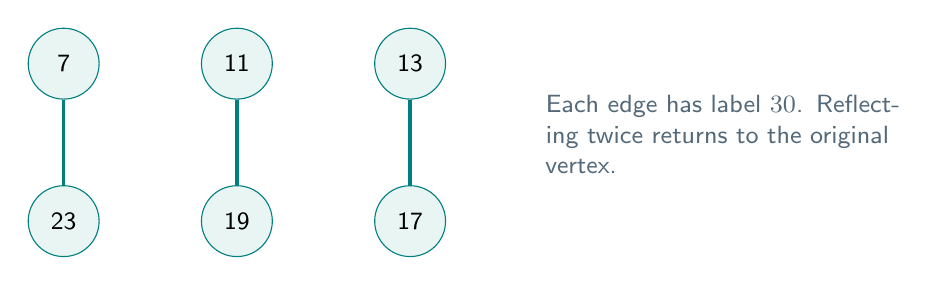
\begin{tikzpicture}[font=\small\sffamily,>=Stealth]
\foreach \i/\x/\a in {0/0/7,1/2.2/11,2/4.4/13}{\node[circle,draw=teal,fill=soft,minimum size=9mm] (a\i) at (\x,1) {\a};}
\foreach \i/\x/\a in {0/0/23,1/2.2/19,2/4.4/17}{\node[circle,draw=teal,fill=soft,minimum size=9mm] (b\i) at (\x,-1) {\a};}
\foreach \i in {0,1,2}{\draw[teal,very thick] (a\i)--(b\i);}
\node[anchor=west,text width=45mm,color=muted] at (6,.1) {Each edge has label $30$. Reflecting twice returns to the original vertex.};
\end{tikzpicture}
\caption{The reflection matching at $N=30$. A loop occurs only when $N/2$ is prime.}
\end{figure}

There is also a spectral form. Take $M>2N$ and a directed Cayley graph on $\mathbb Z/M\mathbb Z$ with an edge $x\to x+p$ for each prime $p\le N$. Its two-step path count from $0$ to $N$ equals $R(N)$. Fourier diagonalization turns this into an exponential-sum identity. But simple expander mixing is too blunt: prime steps have strong local biases, especially parity. Parseval alone forces the largest-eigenvalue bound to be too large for the most naive positivity criterion. A promising spectral argument would need to preserve the \emph{phases} and isolate rational-frequency structure.

\section{A sieve is a covering problem}
For $2\le a\le N-2$, examine the pair $(a,N-a)$. For each prime $\ell\le\sqrt N$, mark $a$ if either coordinate is a nontrivial multiple of $\ell$. The qualification matters: a coordinate equal to $\ell$ is itself prime and must not be crossed out. With that exception in place, an unmarked candidate is exactly a Goldbach representation.

\begin{figure}[htbp]
\centering
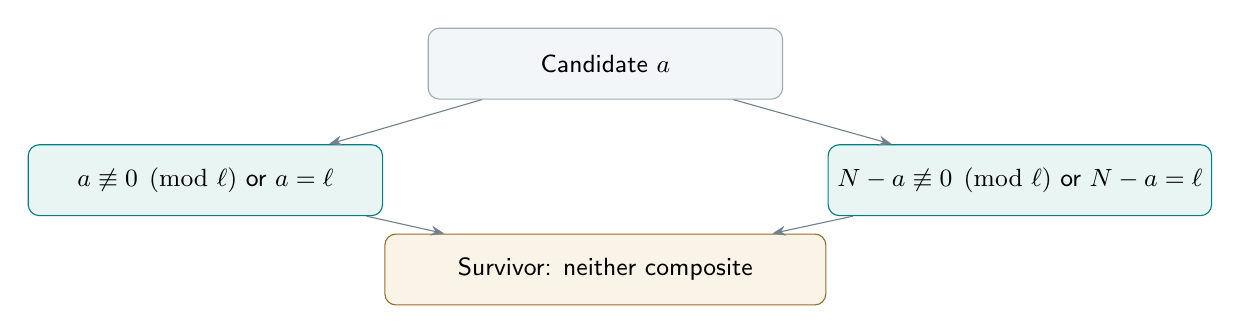
\begin{tikzpicture}[font=\small\sffamily,>=Stealth,node distance=8mm]
\node[draw=ink!40,fill=mist,rounded corners,minimum width=45mm,minimum height=9mm] (c) {Candidate $a$};
\node[draw=teal,fill=soft,rounded corners,minimum width=45mm,minimum height=9mm,below left=of c] (a) {$a\not\equiv0\pmod\ell$ or $a=\ell$};
\node[draw=teal,fill=soft,rounded corners,minimum width=45mm,minimum height=9mm,below right=of c] (b) {$N-a\not\equiv0\pmod\ell$ or $N-a=\ell$};
\node[draw=gold!70!black,fill=gold!12,rounded corners,minimum width=56mm,minimum height=9mm,below=17mm of c] (s) {Survivor: neither composite};
\draw[-Stealth,ink!60] (c)--(a);\draw[-Stealth,ink!60] (c)--(b);
\draw[-Stealth,ink!60] (a)--(s);\draw[-Stealth,ink!60] (b)--(s);
\end{tikzpicture}
\caption{The sieve as a hypergraph cover. Both tests must pass for each sieving prime. A survivor avoids all nontrivial divisibility marks; prime-equals-sieving-prime exceptions are essential.}
\end{figure}

If $Q_z=\prod_{\ell\le z}\ell$, the Chinese remainder theorem gives the exact density over a complete period:
\[
 \delta_N(z)=\prod_{\ell\le z}\left(1-\frac{\nu_\ell(N)}{\ell}\right),
 \qquad \nu_\ell(N)=\begin{cases}1,&\ell\mid N,\\2,&\ell\nmid N.\end{cases}
\]
The period becomes enormous when $z$ approaches $\sqrt N$. A positive density over that period does not guarantee a point in the short interval associated with one $N$. The team checked an average obstruction: at complete-sieve depth, the ratio of the full-period prediction to the actual survivor total tends to $4\e^{-2\gamma}\approx1.260947$. This follows from the prime number theorem, Mertens' product formula and averaging the local factors. It rules out a naive negligible-error approximation, not every possible one-sided lower bound. A closely related two-cloud formulation has appeared in a 2026 preprint \cite{twocloud}.

\section{Chen's bridge and the parity problem}
Chen's theorem offers a particularly sharp distinction between what is known and what remains. Let
\[
 \mathcal C_N=\{p\in\PP:q=N-p\ge2,\ \Om(q)\le2\},\quad
 S_N=|\mathcal C_N|,\quad
 L_N=\sum_{p\in\mathcal C_N}(-1)^{\Om(N-p)}.
\]
A prime complement contributes $-1$ to $L_N$, while a semiprime contributes $+1$. Thus
\begin{equation}\label{eq:chen}
 \boxed{R(N)=\frac{S_N-L_N}{2}}.
\end{equation}
Chen supplies $S_N>0$ for sufficiently large even $N$. The missing step is $L_N<S_N$, a pointwise statement equivalent here to the existence of a prime complement.

A prior version of this programme suggested a fixed relative gap $L_N\le(1-\eta)S_N$ for every large $N$. That target is \emph{false} for the unrestricted set. The prime number theorem and Landau's semiprime asymptotic give, summing over even $N\le X$,
\[
 \sum R(N)\sim\frac{X^2}{2\log^2 X},\qquad
 \sum S_N\sim\frac{X^2\log\log X}{2\log^2 X}.
\]
The aggregate prime share tends to zero like $1/\log\log X$; semiprime complements with a small factor are too numerous \cite{semiprime}. This corrects a proposed target rather than disproving Goldbach.

\section{A roughness threshold and a signed statistic}
Take $z_N=\lfloor N^{1/3}\rfloor$. A number $n\le N$ whose prime factors all exceed $z_N$ has at most two prime factors, counting multiplicity: three would have product exceeding $N$. For ordered pairs $a+b=N$ with both coordinates larger than $z_N$ and free of prime factors up to $z_N$, define counts $PP,PS,SP,SS$ according to whether each coordinate is prime or semiprime.

\begin{center}
\renewcommand{\arraystretch}{1.45}
\begin{tabular}{@{}lcc@{}}\toprule
& \textbf{right prime} & \textbf{right semiprime}\\\midrule
\textbf{left prime} & $PP$ & $PS$\\
\textbf{left semiprime} & $SP$ & $SS$\\\bottomrule
\end{tabular}
\captionof{table}{The four types of cube-root-rough pairs. Reflection exchanges $PS$ and $SP$.}
\end{center}

Let $\liou(n)=(-1)^{\Om(n)}$ and set
\begin{equation}\label{eq:T}
 T(N)=\sum_{\substack{a+b=N,\ a,b>z_N\\ \rough(a),\rough(b)>z_N}}\liou(a).
\end{equation}
The mixed terms cancel by the map $(a,b)\mapsto(b,a)$, so
\begin{equation}\label{eq:Tpair}
 T(N)=SS(N)-PP(N).
\end{equation}
In particular, $T(N)<0$ implies Goldbach at $N$. This is a stronger criterion: $T(N)\ge0$ does not disprove Goldbach.

\begin{theorem}[A signed average; derived in this programme]\label{thm:mean}
As $X\to\infty$, the signed statistic in \eqref{eq:T} obeys
\[
 \sum_{\substack{N\le X\\2\mid N}} T(N)
 \sim \frac{(\log2)^2-1}{2}\,\frac{X^2}{\log^2X}.
\]
\end{theorem}
\begin{proof}[Proof sketch]
At a fixed cutoff $z=X^{1/3}$, the prime number theorem gives $X/\log X$ primes at scale $X$. The number of semiprimes with both factors above $z$ has leading coefficient
\[
 \int_{1/3}^{1/2}\frac{dt}{t(1-t)}=\log2.
\]
Rescaled prime and rough-semiprime counting measures converge to constant multiples of Lebesgue measure. The triangle $u,v\ge0$, $u+v\le1$ has area $1/2$; hence $PP$ has coefficient $1/2$ and $SS$ has coefficient $(\log2)^2/2$. Replacing the fixed cutoff by $N^{1/3}$ changes the sums by lower-order terms; contributions from very small targets can be bounded and then discarded. Equation \eqref{eq:Tpair} supplies the sign. The accompanying research dossier gives the boundary argument.\end{proof}

The constant is negative, about $-0.25977$. Using a classical almost-all Goldbach estimate and a separate finite-residue argument, the research team obtained a lower asymptotic bound of roughly $26.22\%$ for the proportion of even targets satisfying $T(N)<0$. This is a working deduction awaiting external review; it does not exclude an exceptional target. The classical log-weighted estimate used in that deduction is described by Tolev \cite{tolev}.

\begin{caution}{Average is not pointwise}
A negative sum of many values does not make each value negative. Establishing $T(N)<0$ for every sufficiently large even $N$ would itself settle a strengthening of Goldbach. No such estimate is proved here.
\end{caution}

\section{The cutoff where the average changes sign}
Consider a wider family with $z_N=\lfloor N^\alpha\rfloor$, $0<\alpha<1/2$. Let $PP_\alpha$ count prime-prime pairs above the cutoff and $SS_\alpha$ count semiprime-semiprime pairs with all prime factors above it. Their average has a simple coefficient:
\begin{equation}\label{eq:phase}
 \sum_{\substack{N\le X\\2\mid N}}(SS_\alpha(N)-PP_\alpha(N))
 \sim\frac{\log^2((1-\alpha)/\alpha)-1}{2}\frac{X^2}{\log^2X}.
\end{equation}
The sign changes at
\[
 \alpha_*=\frac{1}{1+\e}\approx0.268941.
\]
For every fixed $\alpha<\alpha_*$ the average is positive, forcing $SS_\alpha(N)>PP_\alpha(N)$ for infinitely many even $N$. At the quarter-root cutoff, a scan of 27,986 selected targets through one million found no strict $SS>PP$ instance, despite the asymptotic conclusion. This is a clear example of a convincing finite pattern that cannot persist forever. At $\alpha<1/3$, numbers with three or more factors also survive, so \eqref{eq:phase} compares the two named classes rather than the complete signed survivor set.

\begin{figure}[htbp]
\centering
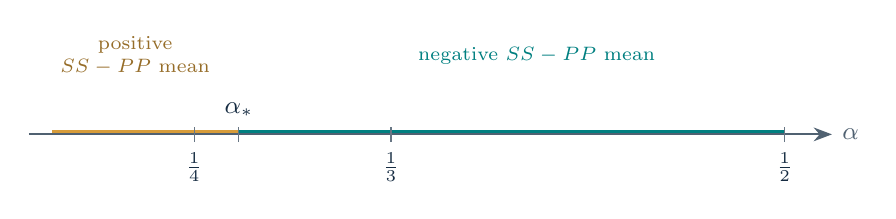
\begin{tikzpicture}[x=30cm,y=1cm,font=\small\sffamily,>=Stealth]
\draw[->,ink!75,thick] (.18,0)--(.52,0) node[right] {$\alpha$};
\draw[gold,very thick] (.19,.04)--(.26894,.04);\draw[teal,very thick] (.26894,.04)--(.5,.04);
\foreach \x/\lab in {.25/{$\frac14$},.33333/{$\frac13$},.5/{$\frac12$}}{\draw[ink!65] (\x,-.10)--(\x,.10);\node[below=3pt,color=ink] at (\x,0) {\lab};}\draw[ink!65] (.26894,-.10)--(.26894,.10);\node[above=3pt,color=ink] at (.26894,0) {$\alpha_*$};
\node[align=center,color=gold!70!black,font=\scriptsize] at (.225,1.0) {positive\\$SS-PP$ mean};
\node[align=center,color=teal,font=\scriptsize] at (.395,1.0) {negative $SS-PP$ mean};
\end{tikzpicture}
\caption{The average balance changes at $\alpha_*=1/(1+\e)$. Only at and above $1/3$ does the four-cell classification exhaust rough survivors.}
\end{figure}

\section{Just below the cube root: three-factor contamination}
For $N^{1/5}<z<N^{1/3}$, let $T$ count prime summands $p$ with $q=N-p>1$ and $\rough(q)>z$. Let $L$ sum $\liou(q)$ over those candidates, and let $H$ count those with $\Om(q)=3$. Five prime factors above $z$ are impossible, so
\begin{equation}\label{eq:triple}
 R_z(N)=\frac{T-L}{2}-H,
\end{equation}
where $R_z$ counts prime complements above the cutoff. A sufficient pointwise inequality is $(T-L)/2>H$. Obtaining it requires a bound on $H$ at the prime-pair scale; the elementary bound obtained in the programme is a logarithm too weak.

For $z=N^\alpha$ with $1/4<\alpha<1/3$, the averaged three-factor count has the coefficient
\[
 c_3(\alpha)=\frac16\!\iint_{\substack{u,v\ge\alpha\\u+v\le1-\alpha}}
 \frac{du\,dv}{uv(1-u-v)}.
\]
This is a classical Buchstab rough-number term, not a new constant \cite{buchstab}. Writing $\alpha=1/3-\varepsilon$, the triangle has side length $3\varepsilon$ and
\[
 c_3(\alpha)=\frac{81}{4}\varepsilon^2+O(\varepsilon^4).
\]
Thus three-factor contamination becomes quadratically small \emph{on average} near the cube-root boundary. The limit in the size parameter is taken first with $\alpha$ fixed. A pointwise inequality still requires new information. A 2026 preprint by Arneth also studies a cubic rough-prime minorant, semiprime cancellation and three-factor contributions \cite{arneth}; its claims have not been independently verified here.

\section{What the graph must know}
Two model obstructions help distinguish a promising graph invariant from an insufficient one. First, consecutive even targets need not share a prime summand. If $C(N)$ counts common summands in representations of $N$ and $N+2$, then for $N\equiv2\pmod6$ and $N\ge8$,
\[
 C(N)=\one_{\PP}(N-3)\left(1+\one_{\PP}(N-1)\right).
\]
Indeed, for $q=N-p>3$, the primes $q$ and $q+2$ must have $q\equiv2\pmod3$, forcing the shared prime $p$ to be $3$. The other possibility is $q=3$. Consequently $C(30k+8)=0$ for every $k\ge1$. Shared-summand constructions have existing antecedents \cite{oeis}.

\begin{insight}{A small formal certificate}
The accompanying file \texttt{GoldbachElementary.lean} was checked with the Lean 4.19.0 kernel. In its explicitly defined elementary divisor-based predicate \texttt{PrimeLike}, the theorem \texttt{no\_adjacent\_common\_summand} verifies for all $k\ge1$ that $30k+8$ and $30k+10$ share no prime summand. The file also checks reflection symmetry, two integer-algebra identities underlying the four-cell and parity counts, and the soundness and completeness of a finite trial-division test. That test certifies the six ordered prime summands for $N=30$. The identities do not formalize the connection between their variables and set cardinalities. This is a certificate for those exact statements, not a verification of Goldbach, the prime-number theorem or the asymptotic deductions in this article.
\end{insight}

Second, one can remove a zero-density subset from the primes while making the remaining set's sumset miss arbitrarily long blocks of even integers. To see the mechanism, average prime-pair counts over short windows in $[X,2X]$, select a window with few total representations, and remove the larger prime in every pair. Repeating this at separated scales removes $o(X/\log X)$ primes but produces growing missing blocks. Hence one-point density and equidistribution in every \emph{fixed} reduced residue class cannot alone force every even sum. Related density results for prime subsets are known \cite{density}.

\section{A precise analytical bridge}
The Fourier and sieve viewpoints meet in the M\"obius-twisted distribution of the reflected sequence $\Lambda(n)\mu(N-n)$. Huang and Li proved that eventual binary Goldbach would follow from specified ordinary and M\"obius-twisted Elliott--Halberstam estimates whose levels add to more than one. Their corollary identifies a twisted level beyond $1/2$ as a sufficient condition with the complementary ordinary input supplied by Bombieri--Vinogradov \cite{huangli}. This is a conditional theorem, not an established estimate of the required strength. A 2026 preprint by Moya identifies a potential moving-endpoint omission in the original derivation and claims a repair under the full maximal-in-$y$ hypothesis \cite{moya}; that criticism and claimed repair have not been independently verified here. Any use of this route must preserve the stated maximal uniformity.

Recent OpenAI mathematics materials and follow-up manuscripts develop multiplicative-function correlations, divisibility graphs and reflected prime-slot methods \cite{oaimath,followups}. These are valuable sources of ideas. Their exact hypotheses must be inspected individually: fixed-form correlation is not automatically uniform in a moving target $N$, and a subexponential roughness cutoff is not automatically a power cutoff. At the cube-root scale the aggregate reflected Liouville bias is nonzero, so a proposed zero relative bias would itself be false. A correctly normalized \emph{one-sided} estimate is the appropriate kind of target.

\begin{insight}{A bridge worth pursuing}
Compare the exact residue-class and modulus requirements of Huang--Li with prime-slot and weighted divisibility-graph estimates. Track the moving target, prime weights, the sieve cutoff, all maxima and the size of every error. The goal is an independently checkable lemma, not a similarity of terminology.
\end{insight}

\Needspace{9\baselineskip}
\section{A programme for the next investigation}
The following tasks are deliberately separated so that one failure does not obscure the others.
\begin{enumerate}[leftmargin=*,itemsep=3pt]
\item \textbf{Audit the deductions.} Check the signed average, moving-cutoff errors, finite-residue density calculation and three-factor integral independently; formalize the elementary identities where feasible.
\item \textbf{Search for countermodels.} Test each proposed uniform inequality against prime-like sequences with the same one-point or low-order statistics. Record the weakest assumption whose removal permits failure.
\item \textbf{Quantify three-factor contamination.} Decompose $H$ in \eqref{eq:triple} by factor ranges, then seek a uniform sieve bound with a constant small enough to leave a positive prime margin.
\item \textbf{Investigate a softer intermediate theorem.} Study whether the rough-semiprime pair count admits an almost-all asymptotic with the appropriate singular series. A proof would require progression uniformity, bilinear minor-arc control and moving-cutoff estimates. It would still leave exceptional targets.
\item \textbf{Build the analytical bridge.} Compare the exact M\"obius-twisted hypothesis in Huang--Li with the strongest applicable prime-slot estimates, including every parameter and dependency.
\end{enumerate}

Christopher Yamba is also developing a complementary approach to the additive structure of the primes, intended for a future follow-up publication. Its specific claims and methods are not assumed in the results above.

\clearpage
\begin{thebibliography}{99}\small\setlength{\itemsep}{0pt}\setlength{\parskip}{0pt}
\bibitem{helfgott} H. A. Helfgott, \emph{The ternary Goldbach conjecture is true}, \href{https://arxiv.org/abs/1312.7748}{arXiv:1312.7748}, 2013.
\bibitem{verification} T. Oliveira e Silva, S. Herzog and S. Pardi, \emph{Empirical verification of the even Goldbach conjecture and computation of prime gaps up to $4\cdot10^{18}$}, Mathematics of Computation 83 (2014), 2033--2060. \href{https://doi.org/10.1090/S0025-5718-2013-02787-1}{doi:10.1090/S0025-5718-2013-02787-1}.
\bibitem{semiprime} D. Cri\c san and R. Erban, \emph{On the counting function of semiprimes}, Integers 21 (2021), \href{https://arxiv.org/abs/2006.16491}{arXiv:2006.16491}.
\bibitem{tolev} D. I. Tolev, \emph{The binary Goldbach problem with arithmetic weights attached to one of the variables}, Acta Arithmetica 142 (2010), 169--178. \href{https://doi.org/10.4064/aa142-2-6}{doi:10.4064/aa142-2-6}.
\bibitem{buchstab} T. Tao, \emph{Probabilistic models and heuristics for the primes}, 2015, \href{https://terrytao.wordpress.com/2015/01/04/254a-supplement-4-probabilistic-models-and-heuristics-for-the-primes-optional/}{rough-number discussion}.
\bibitem{density} A. Alsetri and X. Shao, \emph{Density versions of the binary Goldbach problem}, Acta Arithmetica 218 (2025), 285--295. \href{https://doi.org/10.4064/aa240615-19-9}{doi:10.4064/aa240615-19-9}.
\bibitem{huangli} J.-J. Huang and H. Li, \emph{On the connection between the Goldbach conjecture and the Elliott--Halberstam conjecture}, \href{https://arxiv.org/abs/2005.03811}{arXiv:2005.03811}.
\bibitem{oaimath} OpenAI, \emph{Mathematics research repository}, \url{https://github.com/openai/math}. Statements and formalizations have differing scopes and verification status.
\bibitem{followups} J. Guo, \emph{Follow-ups to the OpenAI mathematics release}, \url{https://github.com/aster2024/openai-math-followups}. Manuscript claims are used as leads with their stated assumptions, not as automatic Goldbach inputs.
\bibitem{moya} R. Moya, \emph{A Moving-Cut Correction to the Huang--Li Conditional Goldbach Argument}, 2026, \href{https://zenodo.org/records/21939906}{Zenodo record 21939906}, preprint; the criticism and proposed repair are unverified here.
\bibitem{arneth} B. Arneth, \emph{A Cubic Prime Minorant and the Remaining Correlation in Binary Goldbach}, 2026, \href{https://zenodo.org/records/23477014}{Zenodo record 23477014}, preprint.
\bibitem{twocloud} G. D. Dura, \emph{Binary Goldbach as a two-cloud complete-sieve survivor problem}, 2026, \href{https://doi.org/10.5281/zenodo.20660791}{doi:10.5281/zenodo.20660791}, preprint.
\bibitem{oeis} OEIS Foundation, \emph{A335045: Minimal common prime of two Goldbach partitions}, \url{https://oeis.org/A335045}.
\end{thebibliography}
\end{document}
